\documentclass[11pt,a4paper]{article}

\usepackage[polish]{babel}
\usepackage[utf8]{inputenc}
\usepackage{polski}
\usepackage[T1]{fontenc}
\usepackage{indentfirst}
\usepackage{wrapfig}    % for wrapping figures, tables

\frenchspacing

%\usepackage{amsmath}
\usepackage{physics}
%\usepackage{bm}
\usepackage{gensymb}
%\usepackage{hepnames}
\usepackage{epsfig}
\usepackage{graphics}
\usepackage[shortlabels]{enumitem}
%\usepackage{xspace}
%\xspaceaddexceptions{[]\{\}}

%
%
%fixpagesize
\pagestyle{empty}
\addtolength{\textwidth}{6cm}
\addtolength{\textheight}{4cm}
\addtolength{\evensidemargin}{-3cm}
\addtolength{\oddsidemargin}{-3cm}
\addtolength{\topmargin}{-2cm}
\parindent=0cm


%
%
%small distance in list/item/enum for enumitem package
\setlist[itemize,enumerate]{topsep=0em}
\setlist{noitemsep}

%print zadanie #
\newcounter{zadanie}\newcommand{\zadanie}[1][]{\addtocounter{zadanie}{1} ~\\  {\bf \emph{Zadanie \arabic{zadanie} #1 }} \\}
\newcounter{zaddom}\newcommand{\zaddom}[1][]{\addtocounter{zaddom}{1} ~\\  {\bf \emph{Zadanie domowe \arabic{zaddom} #1 }} \\}
%\renewcommand{\zadanie}[1][]{\pagebreak  ~\\  {\bf \emph{Zadanie }} \\} \addtolength{\topmargin}{-2cm}

\newcommand{\dbar}{{\mkern3mu\mathchar'26\mkern-12mu d}}


%%%%%%%%%%%%%%%%%%%%%%%%%%%%%%%%%%%%%%%%%%%%%%%%%%%%%%

\begin{document}           % End of preamble and beginning of text.

\begin{centering}
\bf{\Large{Termodynamika z elementami fizyki statystycznej}}\\
Tydzień 11 (19 maja 2023)\\[0mm]
Kombinatoryka, mikrostany, entropia układu izolowanego\\
\end{centering} 
\vspace{5mm}

\zadanie
Gęstość rozkładu prawdopodobieństwa masy truskawek z transportu jest zadana wzorem:\\
$dN = A \cdot m \cdot \exp{(-m/M)} \cdot dm = f(m) \cdot dm$, gdzie parametr $M = 30\,$g.
\begin{enumerate}[a)]
\item Wyznacz stałą $A$.
\item Gdzie leży maksimum rozkładu $f(m)$? Jaka jest średnia waga truskawki?
\item Kontrahent potrzebuje truskawek o masach zawartych pomiędzy 27\,g a 33\,g. Jaki procent truskawek możemy mu sprzedać?
Oszacować wynik jako $f(m)\cdot \Delta m$ i porównać z wynikiem dokładnym otrzymanym przez całkowanie $f(m)$.
\end{enumerate}


\begin{wrapfigure}[7]{r}{0.15\linewidth}\vspace{0mm}
\resizebox{\linewidth}{!}{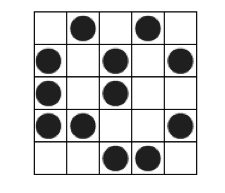
\includegraphics{tydzien10_rys1.png}}
\end{wrapfigure}
\zadanie
Znaleźć liczbę mikrostanów w układzie układu $N$ nierozróżnialnych kulek rozmieszczonych w pudełku z $V$ przegródkami ($V$ oraz $N$ definiują makrostan układu). Wykonać obliczenia dla $V = 20$ i $N = 10$ za pomocą ścisłego wzoru oraz przybliżając wynik używając wzór Stirlinga: $\displaystyle n! \approx \sqrt{2 \pi n} \left(\frac{n}{e}\right)^n$.
\vspace{5mm}

\zadanie
Rozważyć układy $N$ niezależnych cząstek:\begin{enumerate}[a)]
\item klasycznych,
\item kwantowych o spinie całkowitym (tj. bozonów),
\item kwantowych o spinie połówkowym (tj. fermionów).
\end{enumerate}
Zakładając, że pojedyncza cząstka może przebywać w $R$ stanach jednocząstkowych, obliczyć ile wynosi liczba mikrostanów każdego z wymienionych układów.
\\[2mm]
%\small{\em Wskazówka: Zadanie to można sprowadzić do kombinatorycznego problemu rozmieszczania kul w pudełkach. Czą%stki klasyczne należy traktować jako rozróżnialne, natomiast kwantowe jako nierozróżnialne. Poza tym należy wzią%ć pod uwagę, że zgodnie z zasadą% Pauliego żadne 2 czą%stki kwantowe (nierozróżnialne) o spinie połówkowym nie mogą% znajdować się w tym samym stanie jednoczą%stkowym.}\\
%{\em (Zad. 4.4 – A.\,Fronczak, ``Zadania i problemy z rozwiÄ zaniami z termodynamiki i 
%	fizyki statystycznej’’, Oficyna Wydawnicza Politechniki Warszawskiej, 2006).}

\zadanie
Rozważyć układ składający się z dwóch odizolowanych od siebie części: $A$ oraz $B$, 
z których każda zawiera dwie rozróżnialne cząstki mogące przebywać w dyskretnych
stanach energetycznych o energiach będących całkowitą wielokrotnością $\varepsilon$. 
Niech energie podukładów wynoszą odpowiednio $E_A = 5\,\varepsilon$ i $E_B = \varepsilon$. 
\begin{enumerate}[a)]
\item 
Obliczyć ile wynosi liczba mikrostanów $\Omega_{A \cdot B}$ opisanego układu.
\item Jaka będzie liczba mikrostanów $\Omega_{A+B}$ tego układu, jeśli dopuścimy swobodny przepływ
energii pomiędzy podukładami $A$ i $B$ (tzn. usuniemy adiabatyczną przegrodę pomiędzy podukładami)?
\item Przyjmując postulat, że w równowadze termodynamicznej 
wszystkie mikrostany realizujące dany makrostan układu izolowanego są jednakowo
prawdopodobne, obliczyć jakie jest prawdopodobieństwo, że po usunięciu przegrody
energia podukładu $A$ wzrośnie?
\item Jaki podział energii między podukładami $A$ i $B$ jest najbardziej prawdopodobny (tzn. odpowiada stanowi równowagi układu $A + B$)?
\item Znajdź entropię układów $A \cdot B$ i $A+B$. 
\end{enumerate}
%{\em (Zad. 4.5 – A.\,Fronczak, „Zadania i problemy z rozwiÄ zaniami z termodynamiki i
%fizyki statystycznej”, Oficyna Wydawnicza Politechniki Warszawskiej, 2006).}
%\pagebreak

\zadanie
{\em Model Einsteina drgań sieci krystalicznej ciał stałych  (model nieoddziałujących oscylatorów)}\\
Rozważyć układ $N$ rozróżnialnych cząstek, z których każda może przebywać w dyskretnych stanach energetycznych o energiach będących całkowitą wielokrotnością pewnego $\varepsilon$ (tzn. $0,\,\varepsilon,\,2\,\varepsilon,\,3\,\varepsilon$, etc.) --- czyli że są one kwantowymi oscylatorami harmonicznymi. Wyprowadzić wzór na liczbę możliwych stanów (mikrostanow) $\Omega (N, q)$ tego układu realizujących warunek, że całkowita energia układu wynosi $E = q\cdot\varepsilon$. 
Wykonaj przybliżone obliczenia dla $N = 30$ i $q = 30$ przy zastosowaniu wzoru Stirlinga i podaj entropię układu.
\vspace{5mm} 


\zadanie
Rozważyć dwa mogące wymieniać energię układy zawierające $N$ cząstek każdy: $N_A = N_B = N$, 
o całkowitej energii równej $q_A\cdot\varepsilon + q_B\cdot\varepsilon = q\cdot\varepsilon$ (gdzie $\varepsilon$ jest pewnym kwantem energii). 
Stosując model nieoddziałujących oscylatorów oraz zakładając że energia obu podukladów jest duża ($q_i \gg N$), pokazać, że:
\begin{enumerate}[a)]
\item całkowita liczba mikrostanów układu 
      $\Omega_{tot} = \Omega_A \cdot \Omega_B$  
      ma maksimum dla $\displaystyle q_A = q_B = q/2$,
\item $\Omega_{tot}$ w okolicy swego maksimum jest funkcją Gaussa parametru 
      $x$ (gdzie: $\displaystyle q_A = \frac{q}{2} + x$ oraz\linebreak 
      $\displaystyle q_B = \frac{q}{2} - x$),
      której względna szerokość jest rzędu $1/\sqrt{N}$.
\end{enumerate}


\vspace*{1cm}

\begin{wrapfigure}[7]{r}{0.3\linewidth}\vspace{-3mm}
\resizebox{\linewidth}{!}{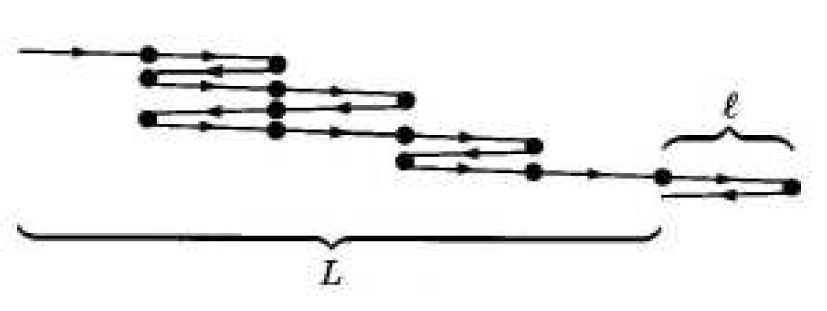
\includegraphics{tydzien10_rys2.png}}
\end{wrapfigure}
\zaddom
Obliczyć entropię jednowymiarowego łańcucha przedstawionego na rysunku, przy założeniu,
że składa się on z $N$ elementów ($N\gg 1$) o długości $\ell$ każdy. 
Przyjąć, że odległość pomiędzy początkowym i
końcowym punktem tego łańcucha wynosi $L$.\\
{\it Odpowiedź: $S=k(\log N!-\log N_+!-\log N_-!)$.}

\zaddom
Rozpatrz dwa izolowane układy rozróżnialnych, nieruchomych i nieoddziałujących cząstek.
Każda cząstka znajduje się w jednym z trzech stanów o energiach:
$-\varepsilon$, 0, $\varepsilon$.
Pierwszy układ (układ {\bf A}) zawiera jedną cząstkę, a jego całkowita
energia wynosi $E_A = \varepsilon$.
Drugi układ (układ {\bf B}) zawiera trzy cząstki, a jego całkowita
energia wynosi $E_B = -\varepsilon$.
\begin{enumerate}[(a)]
\item   Policz liczbę mikrostanów całości złożonej z obu izolowanych układów.
\item   Układy doprowadzono do kontaktu ze sobą tak, że mogą one wymieniać energię.
            Jaka jest teraz liczba mikrostanów?
\item   Ile wynosi teraz najbardziej prawdopodobna energia układu {\bf A}?
\item   Ile wynosi entropia całego układu w punktach a) i b)\,?
\end{enumerate}
{\it Odpowied"z:  a) $\Omega_A=1$, $\Omega_B=6$, ~~ b) $\Omega=19$, ~~ c)   $0$, $S=k\log\Omega$.}

\zaddom
Energia wewnętrzna układu $N$ atomów tworzących $N$-punktową idealną sieć krystaliczną wynosi $U_0$.
Atomy mogą jednak zajmować także miejsca pomiędzy punktami sieci (defekt sieci, takich miejsc dyslokacji też jest $N$).
Atom znajdujący się poza punktami sieci ma dodatkową energię $\epsilon$ i może z równym prawdopodobieństwem wybrać każdy niezajęty punkt dyslokacji.
Znajdź entropię układu, jeżeli jego energia wewnętrzna wynosi $U_0 + n\epsilon$.\\
{\it Odpowied"z: Liczba kombinacji bez powt"orze"n   $\left( \begin{tabular}{c}  N \\ $n$\end{tabular} \right)$.}


% An example of figure placement:
%\begin{wrapfigure}[13]{r}{0.4\linewidth}\vspace{3mm}
%\resizebox{\linewidth}{!}{\includegraphics{NAZWA.png}}
%\end{wrapfigure}
%\zadanie

\end{document}
